\section{EXPERIMENT EVALUATION}
\label{sec:experiment}

In this section, we conduct experiments to evaluate the effect of our proposed solution to mine causality knowledge. All the experiments are implemented in Python and run on a computer with Intel Xeon 32 CPU(2.60GHz) and 173GB memory.

\subsection{Dataset}
The dataset crawled from Chinese financial news website \footnote{\url{ http://finance.sina.com.cn}} contains \textbf{4 991 000} articles, which are split into \textbf{111 330 205} sentences. The number of unique sentences is \textbf{75 572 053}, covering  \textbf{67.88\%} of the total sentences. The number of sentences with casual cue words is \textbf{7 147 141}, covering \textbf{9.46\%} of the total sentences. We can conclude that almost half of the sentences are repetitive, and only tenth sentences express causality explicitly among the unique sentences.

\textbf{Causal patterns statistic.} The elaborate casual patterns can be grouped into 6 groups of templates, and all patterns in one group has different causal words but the same meaning. The matched sentences distribution over these groups of patterns is shown in Table \ref{tab:pattern_statistics}. We can find that the first three rows take most proportion of the whole sentences about 99.21\%. So we will use these three kinds of sentences to extract rule instances.

\begin{table*}[htbp]
	\caption{Number of sentences extracted by causal patterns}
	\begin{center}
		\begin{tabular}{|c|c|c|c|}
			\hline
			\textbf{Pattern template}& \textbf{Pattern}& \textbf{Number}& \textbf{Rate}\\
			\hline
			$A->B$&因为 A,B&2000242&48.32\%\\
			\hline
			$A->B$&A,所以 B&1530311&36.96\%\\
			\hline
			$A->B$&因为 A, 所以B&576851&13.93\%\\
			\hline
			$A_1,A_2->B$&因为 $A_1$, 且 $A_2$, 所以 B&22356&0.54\%\\
			\hline
			$A->B_1,B_2$&因为 A,所以 $B_1$ 且 $B_2$&10178&0.25\%\\
			\hline
			$A_1,A_2->B_1,B_2$&因为 $A_1$, 且 $A_2$,所以 $B_1$  且 $B_2$&1& 0.00\%\\
			\hline
		\end{tabular}
		\label{tab:pattern_statistics}
	\end{center}
\end{table*}	

\textbf{Our newly built Knowledge Base.}
Table \ref{tab:knowledge_base_statistics} shows some statistics of our newly built knowledge base. The number of total Chinese IsA pairs are 515163 which contain concept-instance pairs and concept-subconcept pairs. The number of Chinese concepts is 81082 concluding concepts and subconcepts. The number of instances is 158693. The number of Chinese commonsense pairs is 7316977.\TD{ statistics: instances per concept, concepts per instance }

\begin{table}[htbp]
	\caption{Knowledge Base}
	\begin{center}
		\begin{tabular}{|c|c|}
			\hline
			\textbf{Name}&\textbf{Number}\\
			\hline
			IsA pairs (Taxonomy)&515163\\
			\hline
			Concepts (Taxonomy)&81082\\
			\hline
			instances (Taxonomy)&158693\\
			\hline
			Commonsense Pairs&7316977\\
			\hline
		\end{tabular}
		\label{tab:knowledge_base_statistics}
	\end{center}
\end{table}	

\textbf{Rule.}

Table \ref{tab:rule_statistics} shows that
the number of rule instances extracted from rule instance submodule is \textbf{4 337 755},
the number of candidate rules generalized from rule generalization submodule is \textbf{201 359} and the number of rules specialized from rule specialization submodule is \textbf{42 246}.
We can also conclude the more general these rules are, the less their amount is, since the granularity of knowledge is refining gradually. 

\begin{table}[htbp]
	\caption{derived number of each submodule}
	\begin{center}
		\begin{tabular}{|c|c|}
			\hline
			\textbf{Name} & \textbf{Number}\\
			\hline
			Rule Instances &4337755\\
			\hline
			Candidate Rules &201359\\
			\hline
			Rules &42246\\
			\hline
		\end{tabular}
		\label{tab:rule_statistics}
	\end{center}
\end{table}	

%Rule Instances & 1817014(4337755)\\
%Candidate Rules & 86218(201359)\\
%Rule & 18348(42246)\\


\subsection{Case Study}
Here, we show some mined rules, good rules are shown in Figure \ref{fig:good_rule_case}, and bad rules are shown in Figure \ref{fig:bad_rule_case}. 
\subsubsection{Good Rules}
\begin{figure}[htbp]
	\centerline{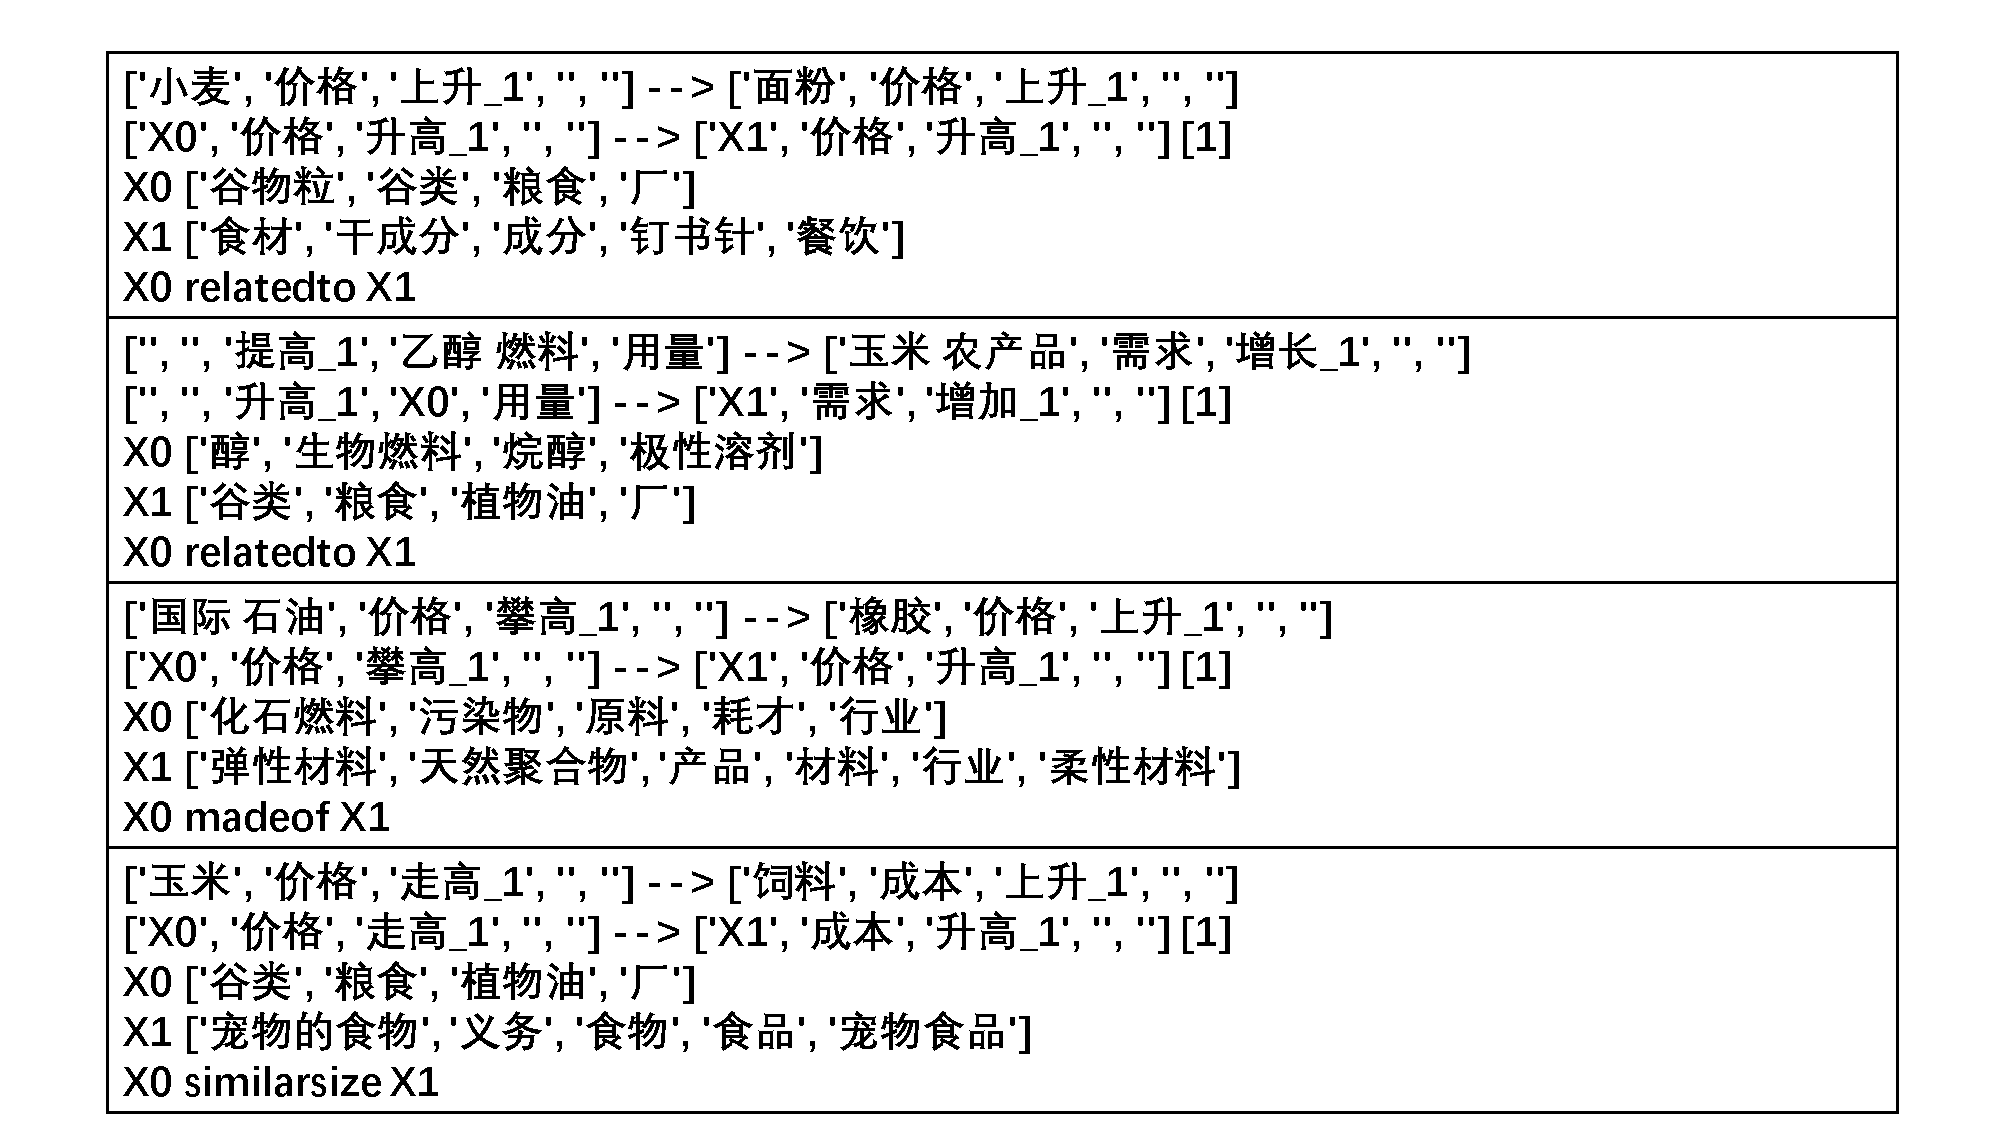
\includegraphics[width=0.9\columnwidth]{figures/good_rule_case}}
	\caption{Good Rule Cases.}
	\label{fig:good_rule_case}
\end{figure}	

Figure \ref{fig:good_rule_case} shows four typically good rules. These rules are pretty readable and quite reasonable.

\TD{Here, we would have a bit more explanation, the "relatedto" relation seems to be less informative, But in fact when considered with concepts together, It will be useful.}

\subsubsection{Bad Rules}
\begin{figure}[htbp]
	\centerline{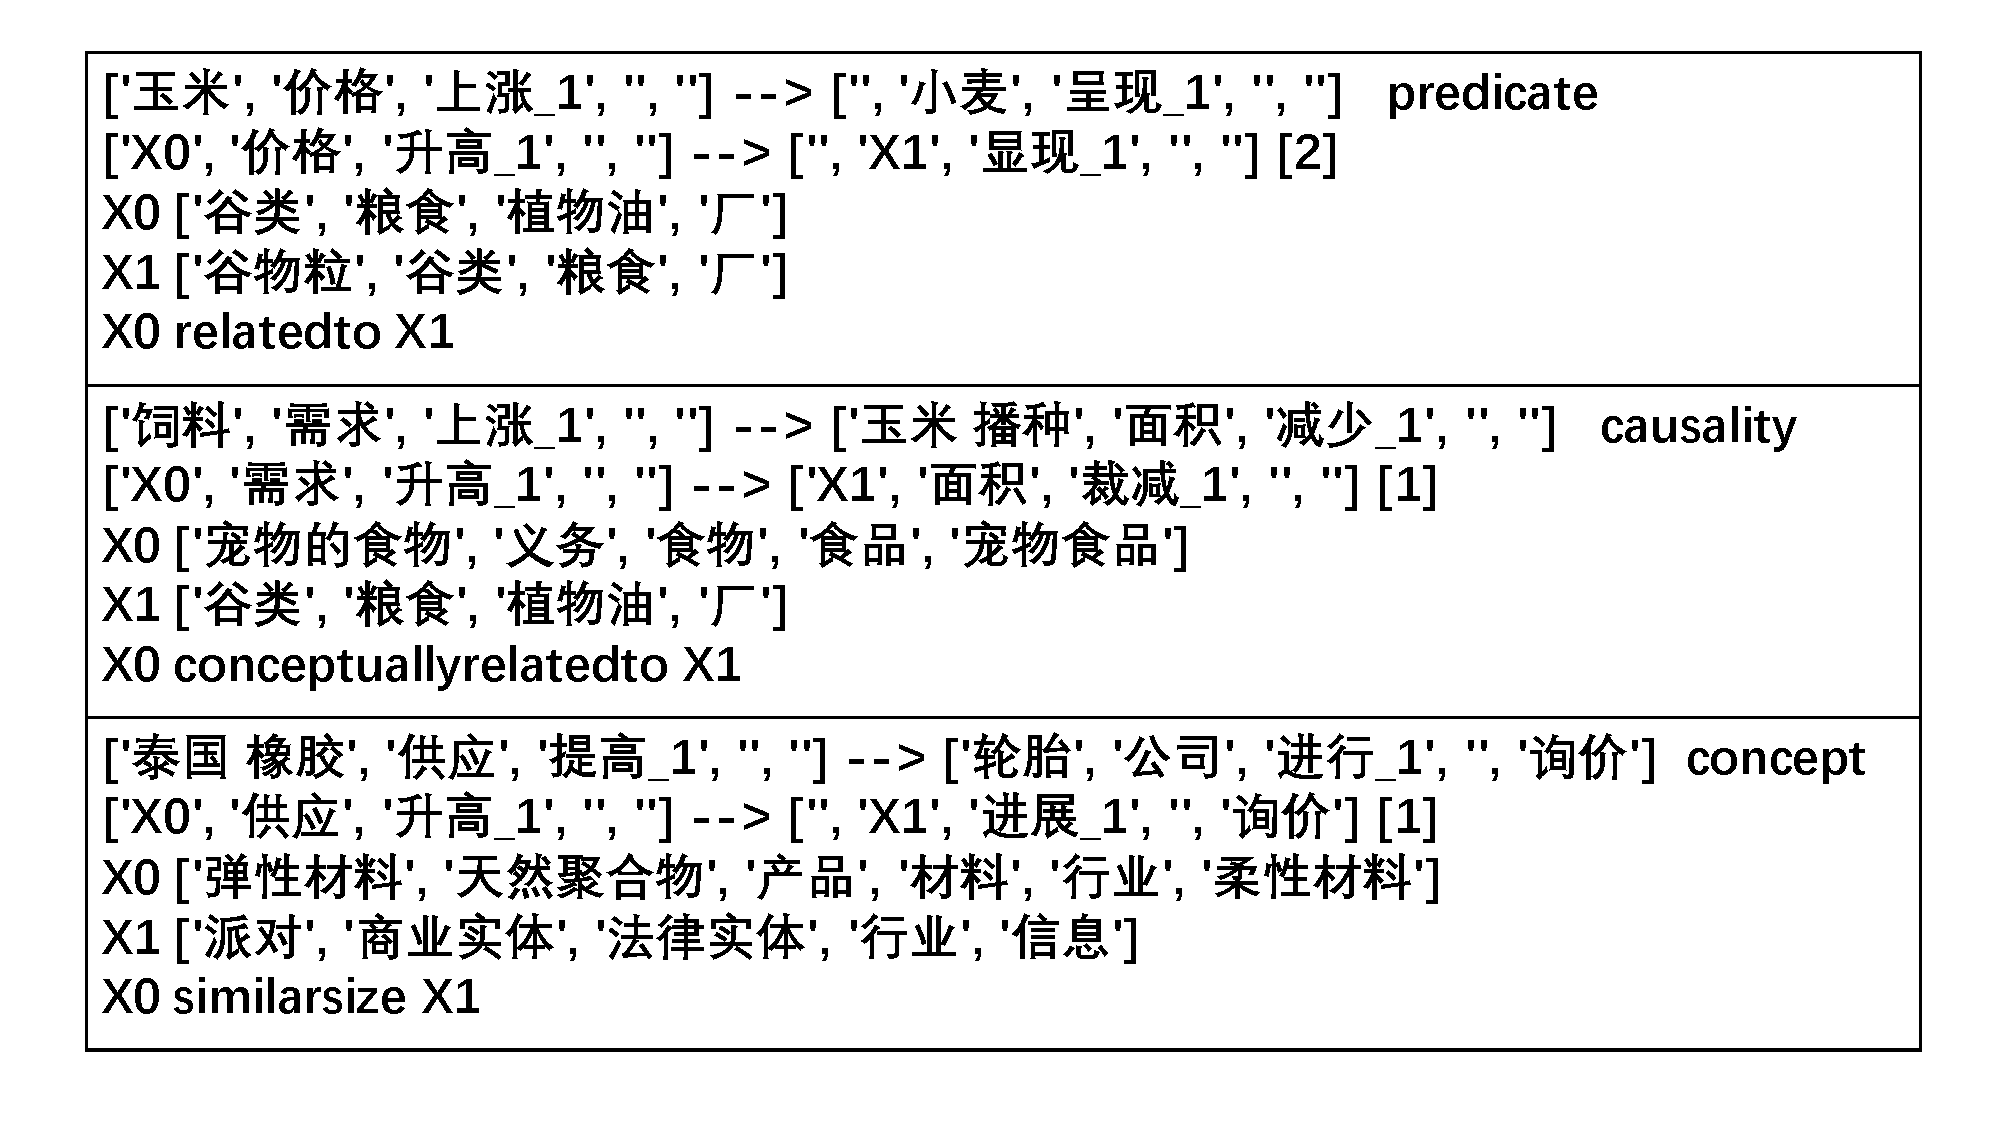
\includegraphics[width=0.9\columnwidth]{figures/bad_rule_case}}
	\caption{Bad Rule Cases.}
	\label{fig:bad_rule_case}
\end{figure}

Figure \ref{fig:bad_rule_case} shows three typically bad rules.
The rule in the first row shows that the effect event is not very well, since it is less informative, and this should be due to event extraction in rule instance extraction submodule.
The rule in the second row shows that the causality between cause event and effect event is not very well which makes this rule unreasonable, and this should be attributed to causal patterns design.
The rule in the third row shows that the '公司' should be not conceptualized, which is already a concept, which is the problem of constructed concrete entities lexicon containing abstract entities.  

	

\subsection{Rule instantiation}
Rule instantiation also called Rule deduction is shown in Figure  \ref{fig:rule_instantiation}, which can be a direct application of the mined causality knowledge.

The method is that given a mined rule derived from our solution, we instantiate this rule into specific rule instances by specializing the concepts into its corresponding specific arguments in the rule. 


\begin{figure}[htbp]
	\centerline{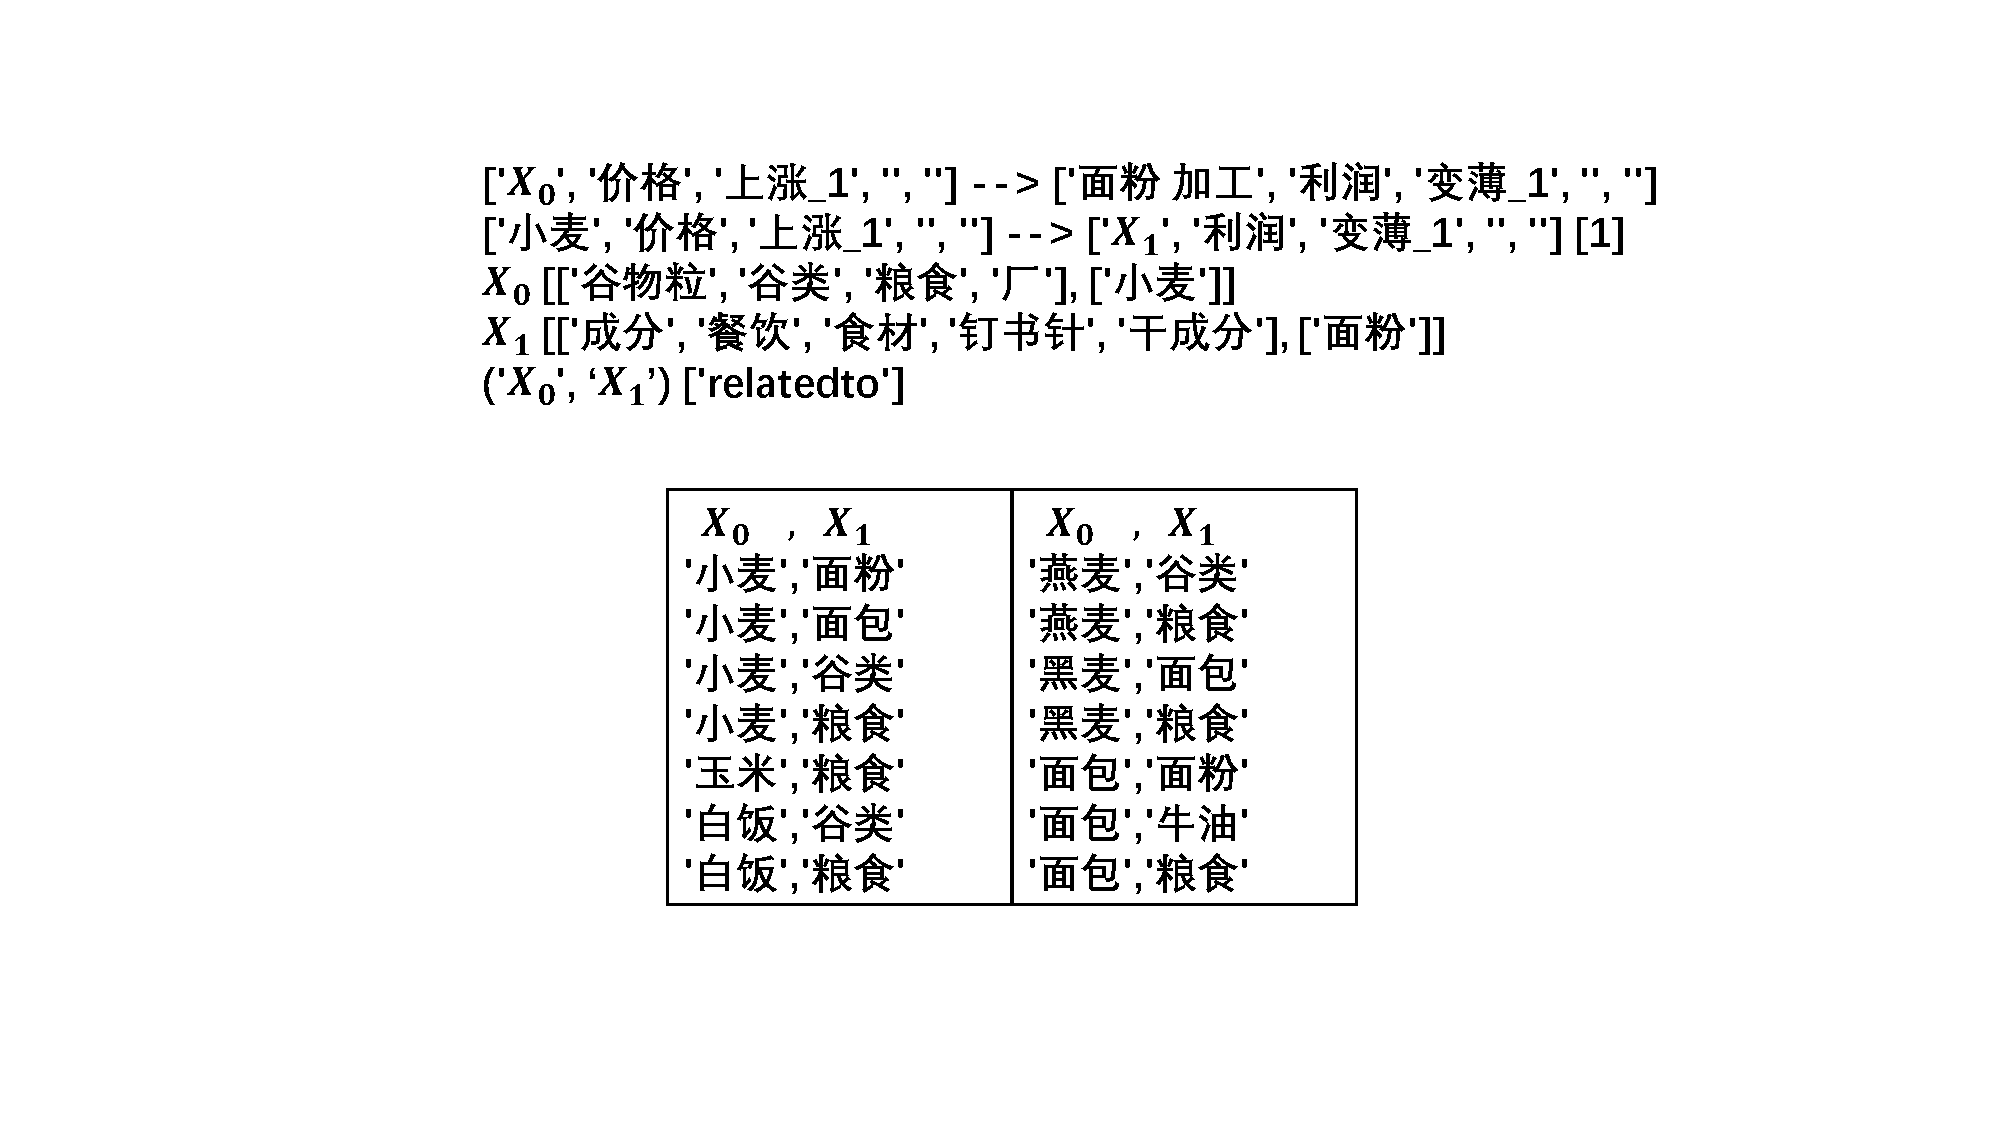
\includegraphics[width=0.9\columnwidth]{figures/instantiation}}
	\caption{Rule Instantiation.}
	\label{fig:rule_instantiation}
\end{figure}


%eveluation metric
%soundness
%complete


%label data for distance supervision in studying causal event extraction
%\textit{Question Answer}
%\textit{Make decision}
